\subsection{Herramientas}

En esta sección presentamos las herramientas utilizadas para este trabajo de investigación.

\subsubsection{Festival y Festvox}

Festival es un framework que permite sistetizar audios, como así tambien una gran variedad de APIs, para el procesamiento de audios y generación de nuevos TTS.

Festvox a su vez expande sobre Festival, agregando todavía mas herramientas relacionadas, que van desde la generación de modelos prosodicos, hasta etiquetado automatico de corpus.

Para este trabajo utilizaremos Festival y festvox para generar los Utternaces requeridos tanto para el entrenamiento como para la sintesis de audios. Estos consisten basicamente en una transcripción fonetica de los audios dividida en segmentos temporales y datos contextuales tales como la cantidad de silabas en la palabra siendo transcripta, fonemas que preceden y proceden al actual, etc.

En particular, Festival tambien cuenta con herramientas de etiquetado automatico. Para este trabajo utilizaremos EHMM alingnment, que a partir de un corpus y sus transcripciones, permite generar utternaces segmentos coinciden con aquellos de los audios.

Estos utternaces serán posteriormente utilizados en el entrenamiento con HTS para modelar cada uno de los fonemas con una mezcla de variables aleatorias gaussianas.

\subsubsection{HTS}

HTS es un TTS basado en HMMs que modela simultáneamente la duración, el espectro (mel-cepstrum) y la frecuencia principal ($f0$) de utilizando un framework de HMM:

\begin{figure}
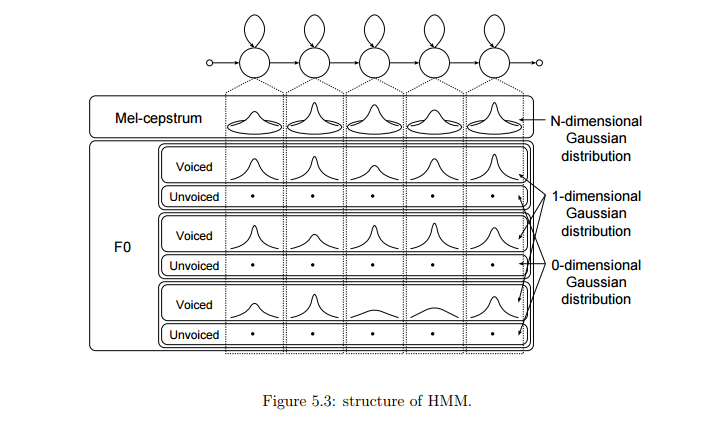
\includegraphics[scale=0.5]{imagenes/hmm.png}
\caption{Estructura de un hmm (simultaneous modeling of phonetic and prosodic parameters, and characteristic conversion for hmm-based text-to-speech systems, takayoshi yoshimura, january 2002)}
\centering
\end{figure}

Por otro lado HTS toma la decisión de modelar la información prosódica dentro de este mismo framework. Para esto, las distribuciones para el espectro, la frecuencia principal y las duraciones son clusterizadas independientemente utilizando la información contextual extraida de los audios de entrenamiento. A continuación se presenta una vista esquemática de la estructura del HMM generado:

\begin{figure}
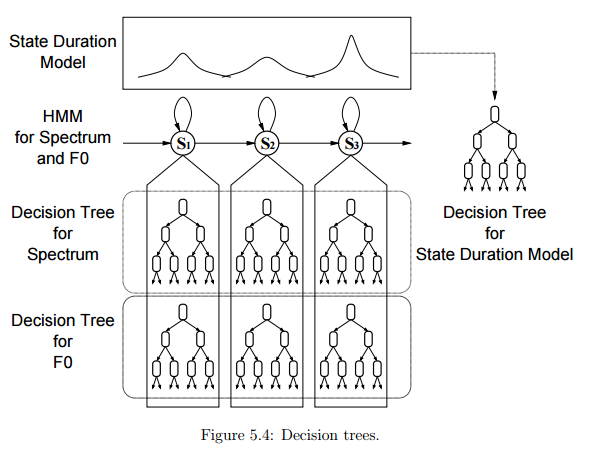
\includegraphics[scale=0.5]{imagenes/hmmContext.png}
\caption{HMM generado (simultaneous modeling of phonetic and prosodic parameters, and characteristic conversion for hmm-based text-to-speech systems, takayoshi yoshimura, january 2002)}
\centering
\end{figure}

En particular para este trabajo la clusterización de datos se realizó generando arboles de decición, para cada fonema se tomaron los dos fonemas precedentes y los dos fonemas procendetes y se extrageron las siguientes features:

\begin{itemize}
\item Modo de articulación del fonema.
\item Punto de articulación del fonema.
\item La perspectiva articulatoria (anterior, central o posterior).
\item Si el fonema es una vocal o una consonante.
\item En caso de ser una vocal, a que categoría pertenecía: por ejemplo para el fonema $/i/: {i, i0,i1}$.
\item En caso de ser una vocal, su Redondeamiento vocálico.
\item En caso de ser una consonante, si es lennis o fortis.
\end{itemize}

En la siguiente imagen se muestra un fragmento de un arbol de decición generado para modelar la duración de los fonemas en un hmm:

\begin{figure}[H]
\begin{center}
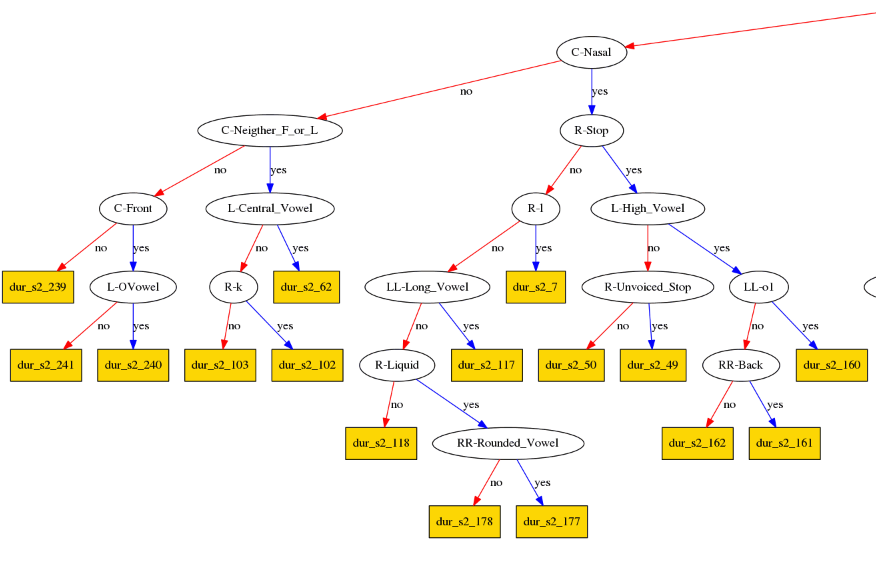
\includegraphics[scale=0.4]{imagenes/arbolDeDesicionTesis.png}
\caption{Árbol de decición generado}
\end{center}
\end{figure}
Con este modelo, el sistema podra inferir por ejemplo cosas como: si el fonema actual no es nasal (C-Nasal) seguido de un stop (R-Stop), que no es el fonema $l$ estará modelado por función de probabilidad gaussiana definida en $dur_s2_7$.

En las primeras iteraciones del desarrollo no contabamos con la información acustica por lo que se generaron modelos carentes de información contextual. En estos primeros modelos se pudo apreciar una calidad mucho peor en los audios generados, sonando estos sumamente metalicos y carentes de prosodia. Tras un par de iteraciónes y tras agregar los factores contextuales pudimos comprobar que ahora las voces sonaban mucho mas humanas.

HTS tambien brinda la posibilidad de realizar speaker-adaptive training. Esta tecnica permite tomar un modelo ya generado y adaptarlo para asimilar caracteristicas de un nuevo hablante. Esta tecnica nace de la idea que conseguir un corpus de datos es costoso tanto en espacio fisico, tiempo de grabación y etiquetado, por lo que a partir de un corpus de datos ya etiquetado y un pequeño corpus nuevo es posible generar una nueva voz sintetica con las caracteristicas del nuevo corpus.

Dentro del adaptative training existen varias tecnicas, en este trabajo utlizaremos offline supervised adaptation, que toma ventaja \dafuk de conocer los utternaces del nuevo corpus. 

% Cosas para hablar:
% contextual factors: cuales son, para que sirven.
% arboles de decición.
% questions
% expandir sobre hmms

\subsubsection{HTS\_engine}

Finalmente para generar voces con acento extrangero se utilizó hts\_engine. Esta herramienta permite interpolar con pesos arbitrarios entre varios modelos para producir un nuevo modelo con una mezcla de la carga fonetica de ambos hablantes y sintetizar audios. Esto nos brinda un gran rango explorativo para experimentar y ajustar la carga fonetica de los modelos originales para acercarnos al objetivo. 


Este metodo tiene a su vez cierto sustento teorico en la manera real en la que un no nativo aprende un idioma con una carga fonetica diferente al nativo. Citando un extracto del trabajo \textit{Transcription of Spanish and Spanish-Influenced English, Brian Goldstein, Temple University}:

\begin{center}
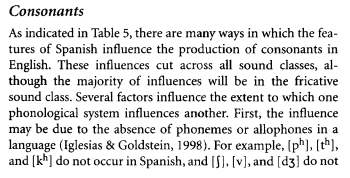
\includegraphics[scale=0.5]{imagenes_investigacion/consonantes1.png}
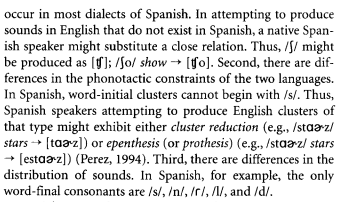
\includegraphics[scale=0.5]{imagenes_investigacion/consonantes2.png}
\end{center}


Visto desde nuestra perspectiva, una persona que aprende una nueva lengua, `interpola' entre aquellos fonemas conocidos y los fonemas `objetivo' de la nueva lengua.


De esta misma manera pero de manera cintetica buscaremos interpolar entre modelos de distintos idiomas buscando de manera artificial ese mismo comportamiento.

\subsection{Entrenamiento}

En esta sección presentaremos la metodología utilizada para el entrenamiento de HMMs y la interpolación entre los mismos.

A modo de resumen, estos serán los pasos a realizar:

\begin{enumerate}

\item A partir de tres corpus de datos, dos de ellos en castellano y uno en ingles, se realizará un etiquetado fonético de los corpus para su posterior utilización en el entrenamiento de los HMMs.

\item Realizar el entrenamiento de los sistemas (Uno por cada corpus disponible). Para esto contaremos con el framework de modelado de HMMs HTS. 

\item Una vez generados los HMMs utilizaremos herramientas provistas por HTS para interpolar entre ellos y así obtener distintos grados de fonética y prosodia inglesa a la hora de sintetizar audios.

\end{enumerate}

Dado que el castellano y el ingles no utilizan los mismos símbolos fonéticos, si queremos sintetizar audios en castellano con el HMM generado con el corpus en ingles, un desafío que deberemos resolver es el de cubrir todos los símbolos fonéticos del castellano por alguno del ingles.

\subsubsection{Preparación De los datos}

Como ya adelantamos, en este trabajo contamos con tres corpus de datos disponibles:

\begin{itemize}
\item \textit{secyt-mujer}: $741$ oraciones, $48$ minutos de habla en castellano.
\item \textit{loc1\_pal}: $1593$ oraciones, $2$ horas y $26$ minutos de habla en castellano.
\item \textit{CMU-ARCTIC-SLT}: $1132$ oraciones, $56$ minutos de habla en ingles.
\end{itemize}

Para los tres corpus se contaba ademas con sus transcripciones grafemicas. 

En los inicios del trabajo contabamos con un solo corpus de datos \textit{secyt-mujer} compuesto por $741$ oraciones equivalentes a $48$ minutos de habla. Para el mismo tambien contabamos con sus transcripciones foneticas y grafemicas anotadas de manera manual.

En primera instancia, realizamos varias pruebas de concepto utlizando HTS y este corpus. Para ello fue neceasrio construir los utternaces del mismo.  

Para obtener los utternaces se plantearon varias estrategias posibles. La primera consistió en utilizar alineamiento automatico utilizando EHMM alignment $[4]$. Los resultados preliminares fueron bastante adversos: los audios generados resultaban poco inteligibles notandose claros defectos acusticos, El mas notable siendo el fonema /rr que se asemejaba mas a una /r.

Utilizando Praat para visualizar el alineamiento entre utternaces y audios, descubrimos que la alineación estaba desfazada. Sospechamos que esto se debió a algun problema con la normalización de los audios.

Dado que para este corpus contabamos con las transcripciones foneticas anotadas de manera manual se procedió a implementar un hibrido con EHMM. De esta manera buscamos mejorar la alineación pero manteniendo el repertorio fonetico, y la metainformación brindada por el alineamiento automatico.

El modelo generado con estos utternaces mixtos resulto ser superior a los generados solo con alineamniento automatico. Aún así los audios sintetizados todavía no alcanzaban una calidad aceptable, sonando metalicos y aguardentosos.

Se pudieron percibir de manera informal otros detalles tales como que la voz original tenía un pitch mayor que la producida por los modelos, al rededor de un $10\%$.

En este momento del trabajo obtenemos otro corpus de datos \textit{loc1\_pal} con $1593$ oraciones en castellano rioplatense que con aproximadamente $2$ horas y $26$ minutos de habla.

Para este corpus no cotabamos con transcripciones foneticas manuales por lo que nos vimos forzados a utilizar EHMM nuevamente. Aún así, los resultados fueron muy superiores a los conseguidos con \textit{secyt-mujer}. Los audios sintetizados resultaban inteligibles y con un marcado acento rioplatense. Tras algunas pruebas de concepto donde se experimentó con varios valores de GAMMA, rango de las frecuencias principales, y otros parametros que concideramos podían afectar la calidad de la voz decidimos que la voz ya había alcanzado la calidad adecuada para proseguir con el resto del trabajo.

Especulamos que la disparidad en la calidad de los resultados es causada principalmente por la cantidad de audios y horas de habla de cada corpus. Concideramos que esto juega un papel predominante en la calidad de los TTS generados, aún cuando se utiliza un metodo de etiquetado puramente automatico y propenso a errores en el alineamiento.

Por ultimo utilizamos el corpus \textit{CMU-ARCTIC-SLT} con $1132$ oraciones y $56$ minutos de habla, disponible en la pagina de hts [5].

Para este trabajo todos los audios usarán sampling rate de 48kHz, precisión de 16 bits, mono.

El rango de extraccion de frecuencia principal para  utilizado fue de 100 hz a 350hz.

Una lista extensiva de los parametros utilizados para el entrenamiento se puede ver en el apendice 3

% hablar de intelibililidad como para ya ir adelantando el tema
% Cosas para hablar:
% 5 fonemas.
%TODO: phonetically balanced?
% desarrollar generacion de uternaces: secty alineaminento mixto: tiempos a mano, features automaticos.

\subsubsection{Repertorio Fonetico y Mapeo De Fonemas}

%hablar un poco mas de utternaces.

Para las transcripciones foneticas, tanto de los audios en ingles como en castellano, utilizamos los repertorios foneticos brindados por festvox (ver apendice 1).

El primer desafío que se presenta es que estos repertorios foneticos no tienen un mapeo directo con el Alfaveto Fonetico Internacional: por ejemplo con este repertorio fonetico, en el castellano existen tres fonemas distintos para la /i/. Consideramos que esta decición por parte de festvox proviene de la necesidad de poder diferenciar la /i/ acentuada de la no acentuada y de aquella presente en los diptongos. 

Por otra parte, surge aquí un problema: como sintetizar oraciones en castellano utilizando un repertorio fonetico distinto, donde incluso la cantidad de fonemas es diferente. Como solución a esto desarrollamos de manera perceptual e iterativa, un mapeo del ingles al castellano en el que cubriremos cada fonema del castellano por al menos uno del ingles. El mapeo que concideramos devolvió los mejores resultados puede observarse en el apendice.

Los fonemas marcados como notUsed los consideramos lo suficientemente diferentes como para no mapearse a nigun fonema del castellano.

Ademas para completar el repertorio, se tomaron la mitad de los fonemas /r/ y se remplazaron con /rr/ y de manera similar se tomaron la mitad de los fonemas etiquetados como /hh/ y se remplazaron con /g/.

Utilizamos este mapeo para generar un tts en ingles capaz de sintetizar oraciones en castellano. Por supuesto los resultados obtenidos sintetizando audios de esta manera generan audios incomprensibles y de muy baja calidad.

En el proximo paso procederemos a realizar mezclas entre el tts en castellano y el tts presentado aquí para generar un nuevo tts donde se pueda hacer un ajuste gradual de cada uno de estos modelos. 

% mapeo utilizado mostrar.
% el etiquetado de cmu\_arctic es en ingles y mapeando al castellano.

\subsubsection{Interpolación entre modelos}

Una vez generados ambos modelos con fonemas `similares' proseguimos realizando pequeñas pruebas internas para probar la efectividad del metodo y concluimos que eran satisfactorias, fue posible generar oraciones donde la carga fonetica podía reconocerse como estadounidense (detalles distintivos como la /r mas suavizada, o las vocales mas abiertas).


\subsubsection{Speaker-adaptive Training}

Se realizaron varias pruebas de concepto donde habiendo entrenado un HMM con \textit{CMU-ARCTIC-SLT} se le realiza speaker adaptation con el corpus de \textit{loc1\_pal}, pero resultaron no concluyentes. El HMM final perdía completamente las caracteristicas y el acento de \textit{CMU-ARCTIC-SLT} por lo que se decidió no proseguir por este camino. 
% Cosas para hablar:
% Expandir en que consiste la interpolación.
